\documentclass[Orbiter User Manual.tex]{subfiles} 
\begin{document}

\section{Extra functionality}
%TODO add section link
The standard Orbiter installation comes with a set of optional plug-in modules which can be used to enhance the core functionality of the simulator. To enable these additional functions, the appropriate modules must be loaded in the \textit{Modules} tab of the Orbiter Launchpad dialog (see TODO on how to activate plug-in modules).\\
Many more plug-ins are available from 3$^{rd}$ party add-on developers. Check out the Orbiter repositories on the web to find more.\\
You should only activate modules you want to use during your simulation session, because many plug-ins may consume CPU cycles even if they are running in the background. Too many active modules can degrade the simulation performance.\\
%TODO add section link
When activated, some plug-ins, such as custom MFD modes, take effect automatically whenever the simulation is started. Others are accessible via the \textit{Custom functions} dialog (see TODO).


\subsection{Scenario editor}
Orbiter comes with an editor that allows creation, configuration and deletion of vessels from within a running simulation session, as well as adjustment of simulation time. The editor is provided as a plug-in module. To use it, make sure that the \textit{ScnEditor} module is activated in the Modules tab of the Orbiter Launchpad dialog.

\begin{figure}[H]
	\centering
	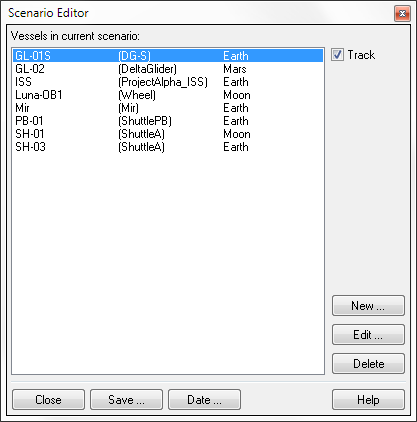
\includegraphics[width=0.4\hsize]{scn_editor.png}
\end{figure}

\noindent
During the simulation the editor can be accessed by opening the \textit{Custom functions} dialog with \Ctrl\keystroke{F4} and double-clicking the \textit{Scenario Editor} entry in the list. This brings up the editor’s main page. From here, you can either configure or delete any vessels currently present in the simulation, or create a new vessel.\\
%TODO doc link, copy?
The operation of the scenario editor is described in detail in a separate document: TODO. This also contains a section for vessel add-on developers who want to add customised scenario editor support to their vessel code.


\subsection{External MFDs}
If the multifunctional displays (MFD) integrated in the vessel instrument panels do not provide enough information, you can open additional MFD displays in external windows. This is particularly useful in multi-monitor settings where you can display the Orbiter simulation window on one monitor, and a set of MFDs on the other.

\begin{figure}[H]
	\centering
	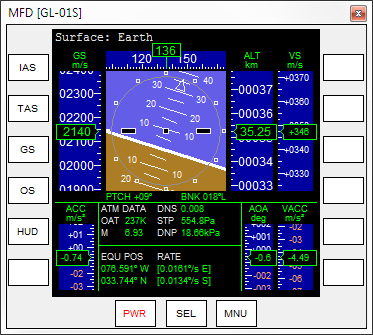
\includegraphics[width=0.4\hsize]{ext_mfd.png}
\end{figure}

\noindent
To open external MFDs, the \textit{ExtMFD} module must be activated in the Orbiter Launchpad dialog. You can then open any number of MFD windows by clicking \textit{External MFD} from the Custom functions dialog (\Ctrl\keystroke{F4}).\\
%TODO add section link
External MFDs behave in the same way as built-in MFDs. They can be controlled by pressing the buttons around the left, right and bottom edges. See TODO for a description of the available MFD modes and controls.\\
Unlike built-in MFD displays, the window MFDs can be resized. They are available in external view as well as cockpit view, and they can be configured to either automatically follow the focus vessel, or remain attached to a specific vessel, even if the focus is switched to a different vessel.


\subsection{Performance meter}
This is a dialog box to keep track of Orbiter’s frame rate performance and simulation time step intervals. It shows the frames per second (FPS) and/or the step length interval (in seconds) between consecutive frames in a graphical display over the last 200 seconds. This is a useful tool to estimate the impact of complex scenery and visual effects on the simulation performance. The time step graph also incorporates the effect of time acceleration, and thus reflects the fidelity of the physical model (accuracy of trajectory calculation, etc.)

\begin{figure}[H]
	\centering
	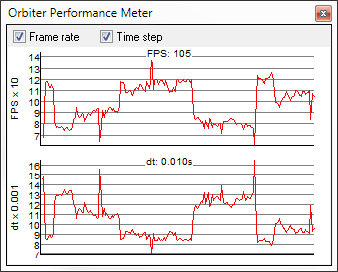
\includegraphics[width=0.4\hsize]{perf_meter.png}
\end{figure}

\noindent
This function is available if the \textit{Framerate} module is active and is accessible via the \textit{Frame Rate} entry in the Custom functions list (\Ctrl\keystroke{F4}).


\subsection{Remote vessel control}
The Remote Vessel Control plug-in allows remote control of the engines of any spacecraft in the simulation.

\begin{figure}[H]
	\centering
	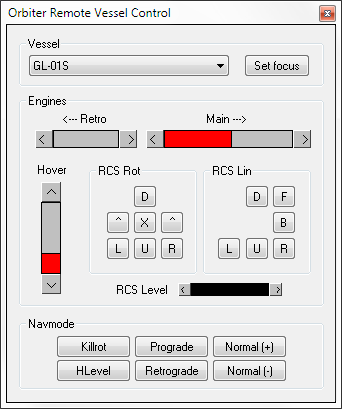
\includegraphics[width=0.4\hsize]{rcontrol.png}
\end{figure}

\noindent
The dialog allows selection of a vessel from a drop-down list. It contains gauges for main, retro and hover engines, controls for RCS thrusters in rotational and linear mode, and provides access to the standard attitude control functions. RCS thrust can be controlled with a slider. This interface can also be useful if simultaneous access to linear and rotational RCS modes is required.\\
This tool is available if the \textit{Rcontrol} module is active and can be accessed via the \textit{Remote Vessel Control} entry in the Custom functions list (\Ctrl\keystroke{F4}).


\subsection{Flight data monitor}
The \textit{Flight data monitor} graphically displays a number of flight parameters as a function of time. This tool is available if the \textit{FlightData} module is active. The dialog box is accessible via the Custom functions list (\Ctrl\keystroke{F4}).

\begin{figure}[H]
	\centering
	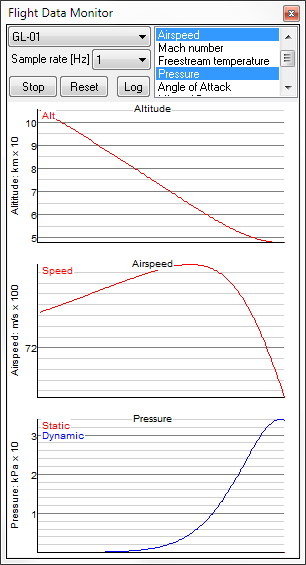
\includegraphics[width=0.3\hsize]{flight_data_monitor.png}
\end{figure}

\noindent
The control area of the dialog box allows selection of the vessel for which data are displayed, sampling rate, and the set of data to show.\\
The following parameter displays are supported:

\begin{itemize}
\item Altitude
\item Airspeed
\item Mach number
\item Free stream temperature
\item Static and dynamic pressure
\item Angle of attack
\item Lift and drag force
\item Lift over drag ratio (L/D)
\item Vessel mass
\end{itemize}

\noindent
For each parameter category selected in the list, a graph display is opened below the control area to track that parameter as a function of time.

\begin{itemize}
\item The Start/Stop button starts or stops the update of the data graphs.
\item The Reset button clears the data graphs.
\item The Log button starts or stops the output of flight data to a log file. When the Log button is ticked, Orbiter writes out data into text file FlightData.log in the main Orbiter directory. This file can later be used to analyse or visualise the data with external tools. FlightData.log is overwritten whenever Orbiter is restarted.
\end{itemize}


\subsection{Lua Console}
%TODO add section link
The \textit{Lua Console} window is available from the Custom functions list (\Ctrl\keystroke{F4}) if the \textit{LuaConsole} module has been activated. The console provides an interactive script interface which allows script execution (tutorials, autopilots, etc.) and reading/writing of simulation and spacecraft parameters and states. The script interface and Orbiter Lua extensions are described in more detail in TODO.

\begin{figure}[H]
	\centering
	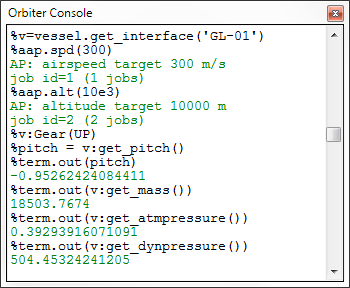
\includegraphics[width=0.4\hsize]{console.png}
\end{figure}


\end{document}
